\section{Kanchanaburi}

Date: 12/06/2008

%\begin{multicols}{2}

Avant de commencer la lecture, avez vous lu l'article sur Bangkok que je viens d'écrire? (oui je fais les articles deux par deux maintenant, allez savoir pourquoi).

Kanchanaburi vous connaissez ? Mais si, faites un effort...

Bon je vais poser la question autrement : Le pont de la rivière Kwai, vous connaissez? Allez pour ceux qui n'ont pas vu le film, bref rappel historique : Nous sommes en cinquante avant Jesus Christ, heu non, là je me trompe d'histoire... Le pont à été construit par les Japonais pendant la seconde guerre mondiale. Enfin quand je dit par les Japonais je devrais plutôt dire par leur prisonniers. 9.000 prisonniers sont morts durant sa construction, ce qui est particulièrement étonnant quand on voit la taille du pont. Le film, lui, a eu 6 oscars et reste le 13ème film le plus vu au monde.

Je suis allé à Kanchanaburi pour voir le pont du film, non pas pour dire "j'y étais", mais plus car dans le film le pont a l'air vraiment impressionnant, et puis tant qu'à être dans le coin.... Seulement c'est un faux!!! En vrai le pont ne fait pas plus d'une cinquantaine de mètres, il est en béton et en fer, non pas en bois. Assez parlé, je vous le montre.

\hspace*{-0.45cm}
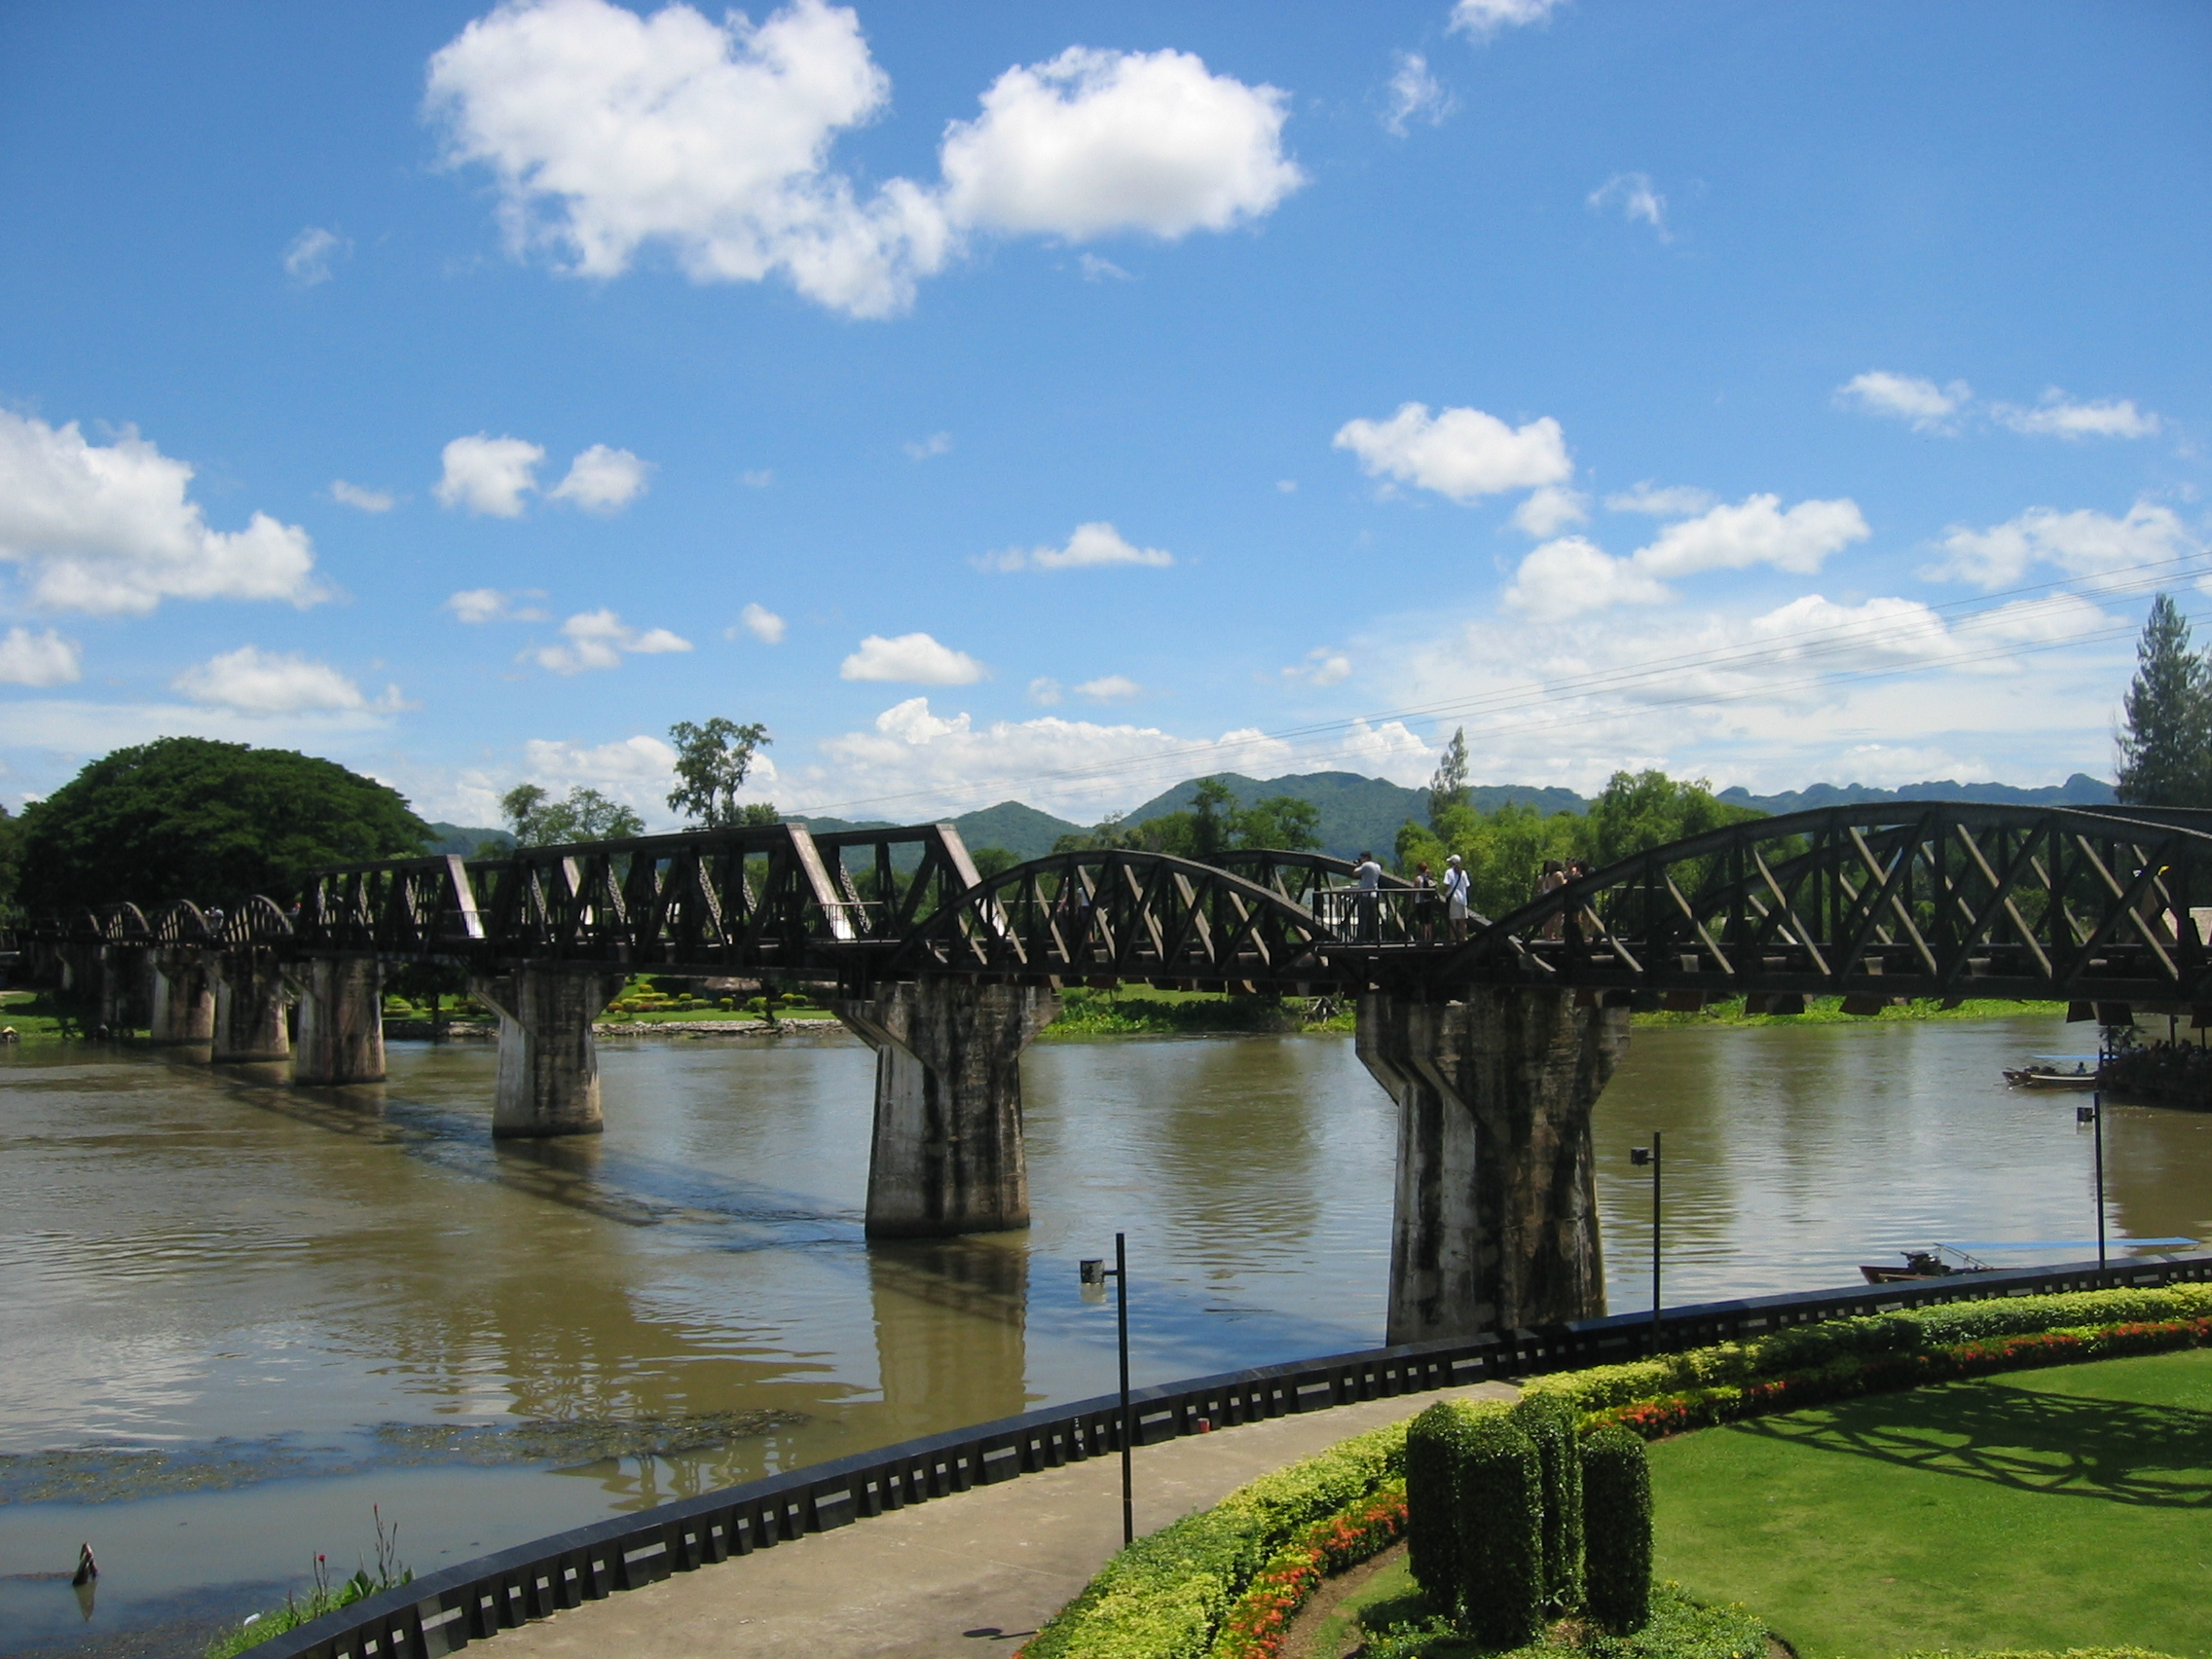
\includegraphics[width=9.7cm]{articles/Kanchanaburi/1400.jpg}
Le pont de Kanchanaburi.

\hspace*{-0.45cm}
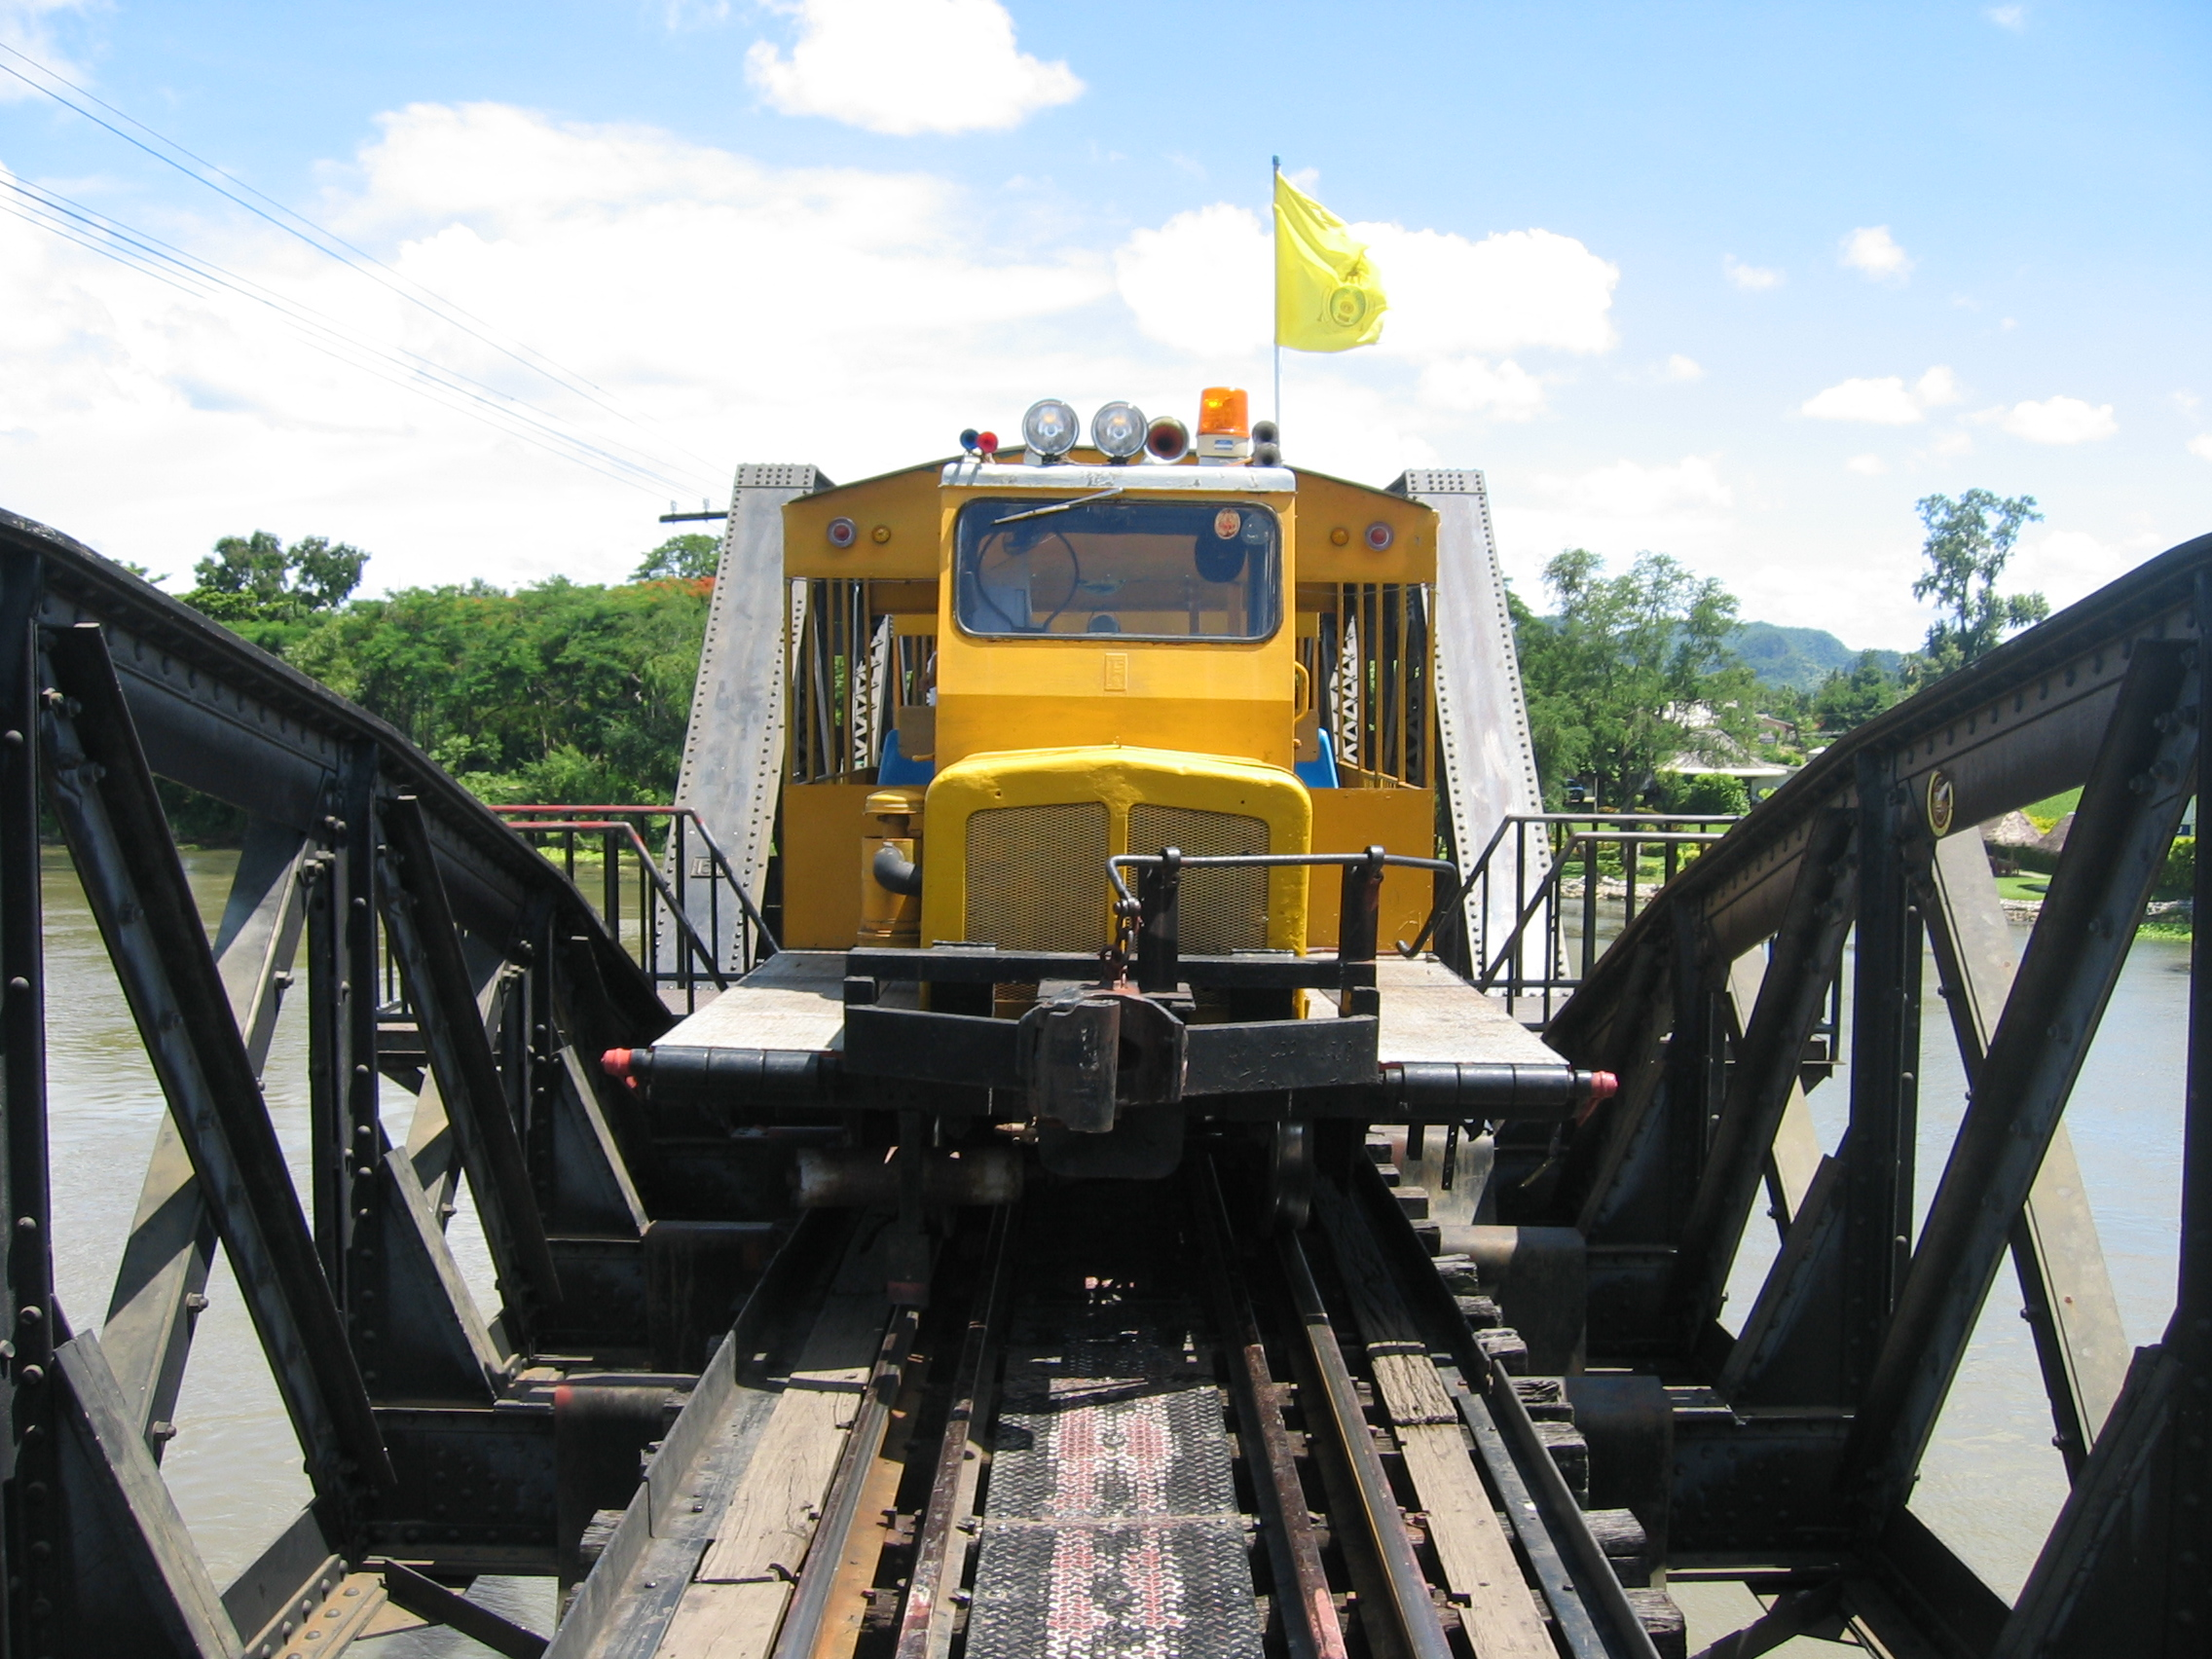
\includegraphics[width=9.7cm]{articles/Kanchanaburi/1401.jpg}
Le train qui passe sur le pont.

Petite déception pour Kanchanaburi, donc. d'autant plus que je ne suis pas le seul à me faire avoir, au final la ville est remplie de touristes, la rivière est remplie de speed boats qui font un max de bruit. Y'a même des boîtes de nuit flottantes... Y sont fous ces romains!!!

Va falloir faire autre chose de sympa dans le coin, car même en louant une motor bike je n'ai pas vraiment été séduit par les alentours. Je propose les chutes d'eau d'Erawan, à deux heures de bus de là, vous êtes d'accord?

Juste avant de partir j'ai rencontré deux francaises bien sympas (là je fais le faux jeton passqu'elle m'ont promis qu'elles passeraient voir ce blog, Anna et Geraldine, si vous me lisez...) qui arrivaient juste et qui ne savaient pas trop où aller en premier, nous sommes donc allés à Erawan ensembles.

Ces chutes sont sur 7 niveaux où il est possible de se baigner. Inutile d'en dire plus, je vous laisse regarder.

\hspace*{-0.45cm}
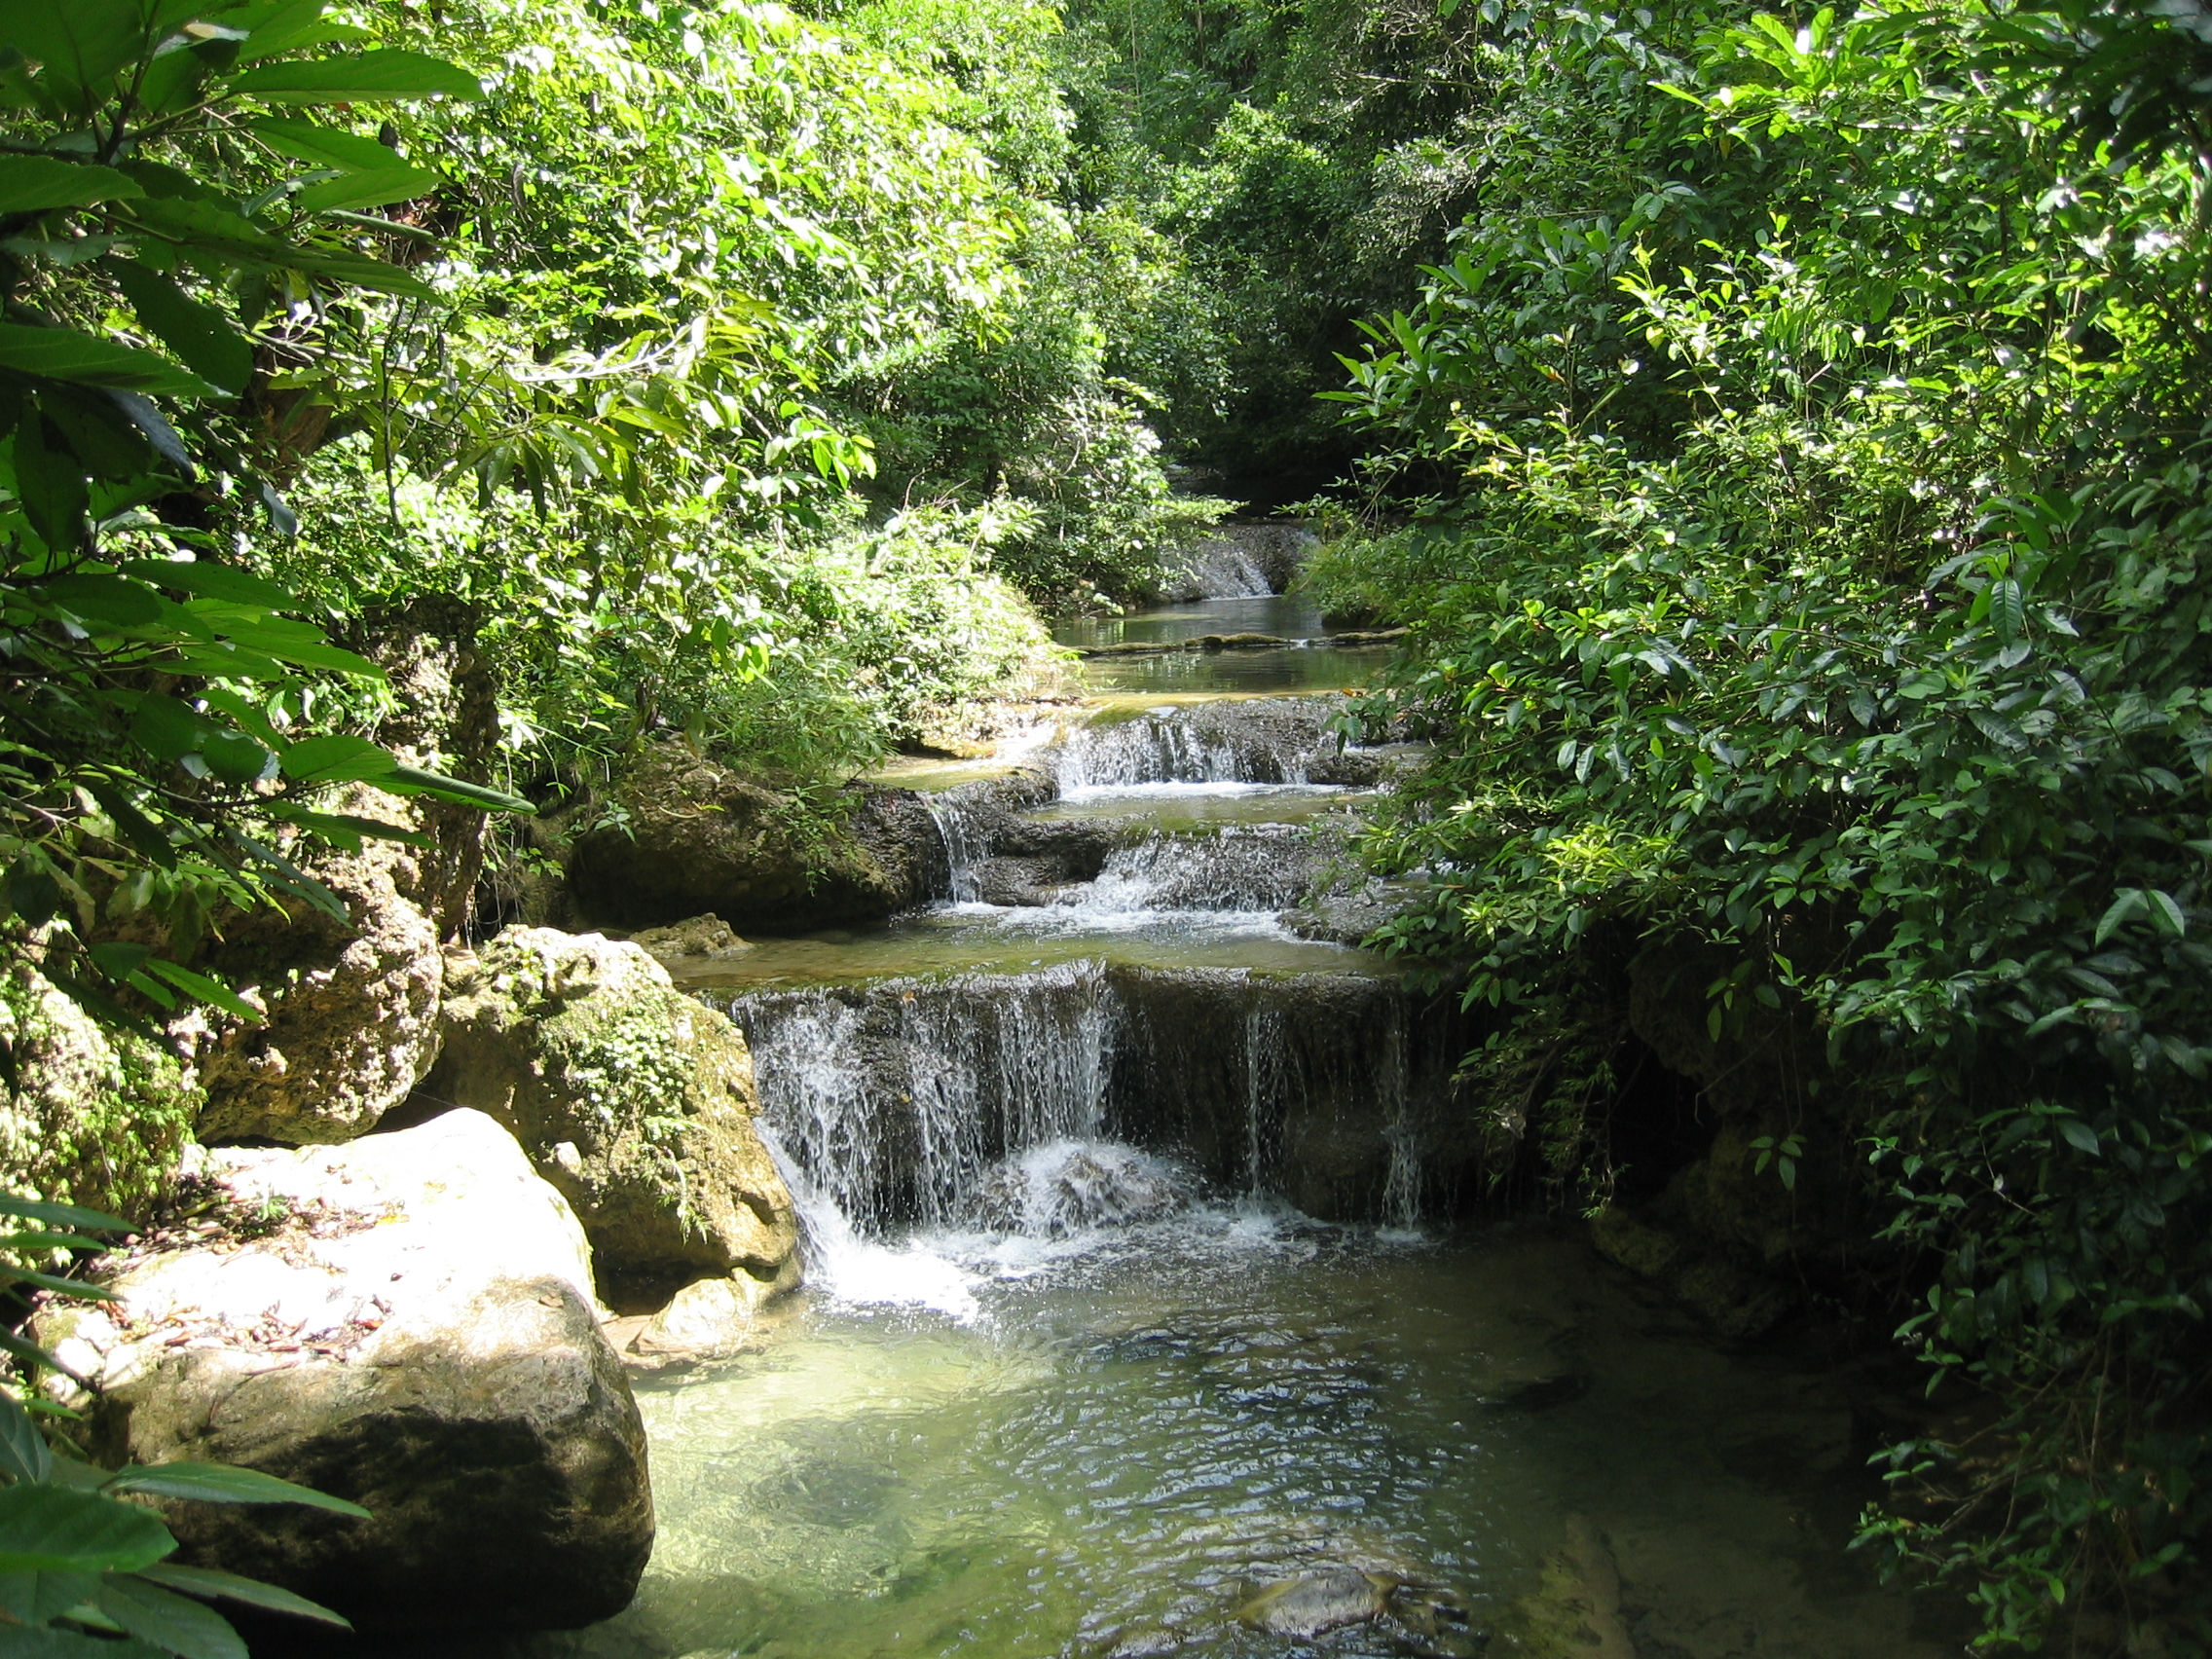
\includegraphics[width=9.7cm]{articles/Kanchanaburi/1440.jpg}
Les chutes d'Erawan.

\hspace*{-0.45cm}
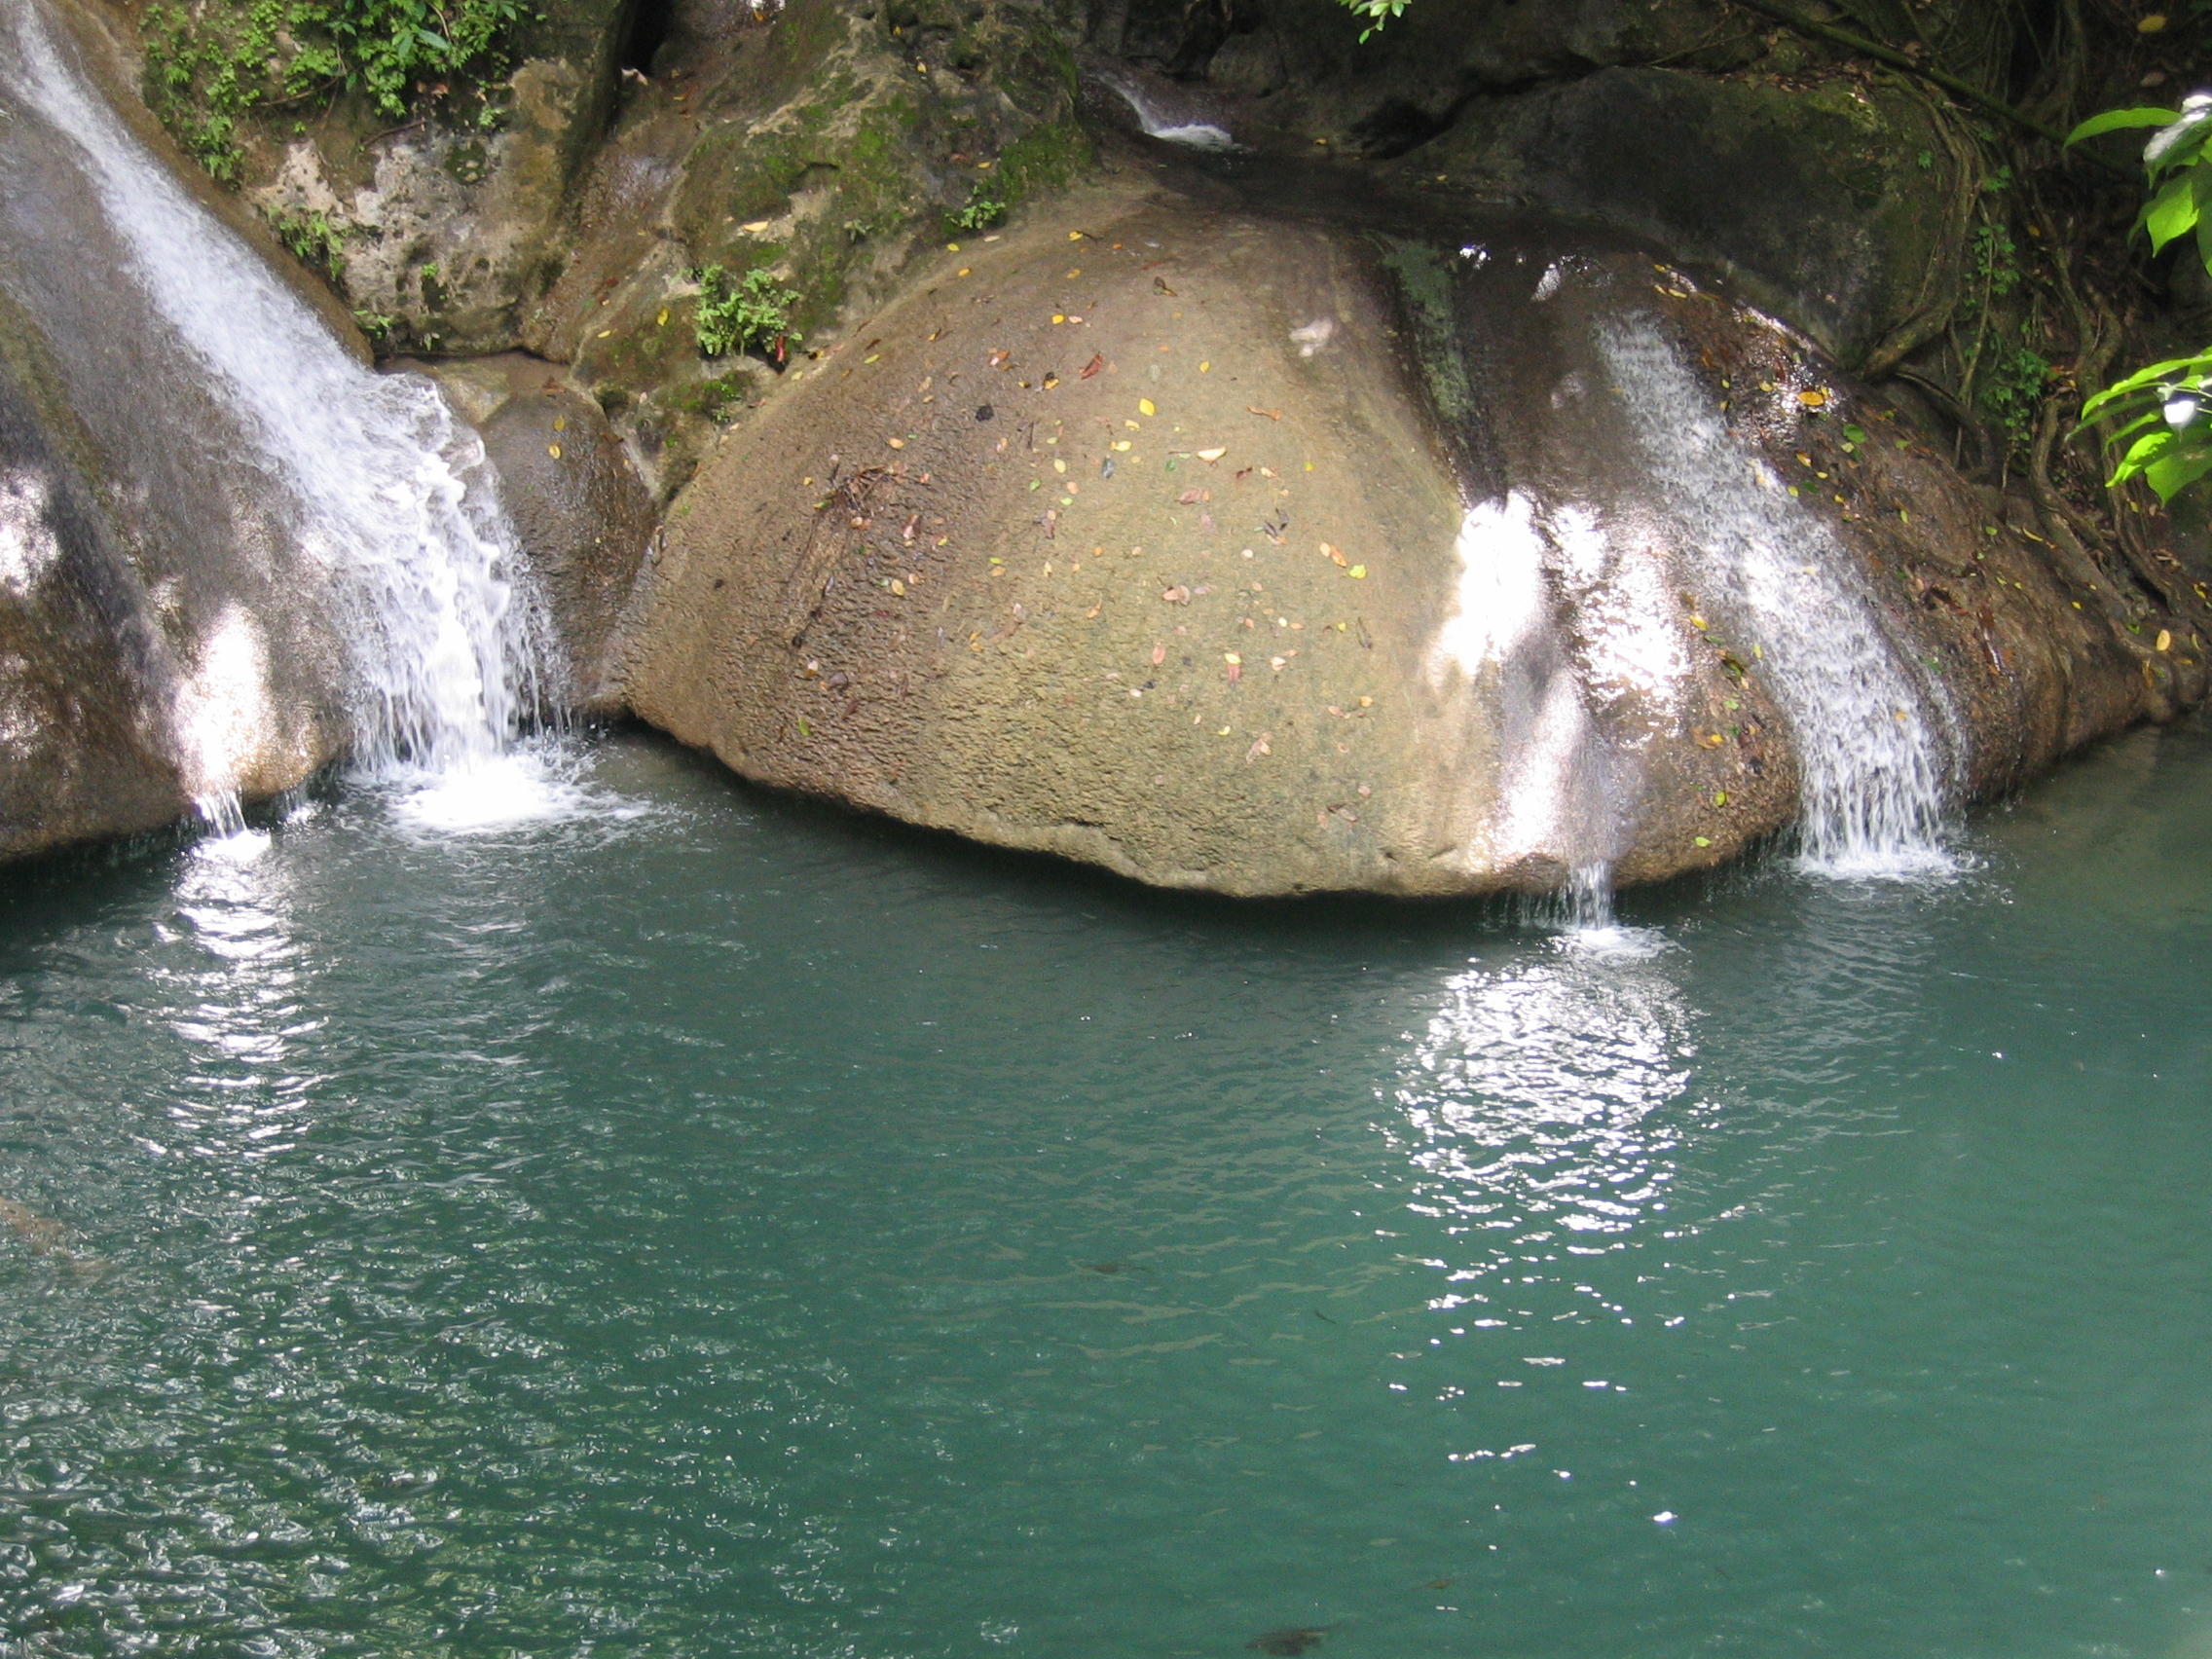
\includegraphics[width=9.7cm]{articles/Kanchanaburi/1439.jpg}
L'est pas bizarre ce rocher ?

\hspace*{-0.45cm}
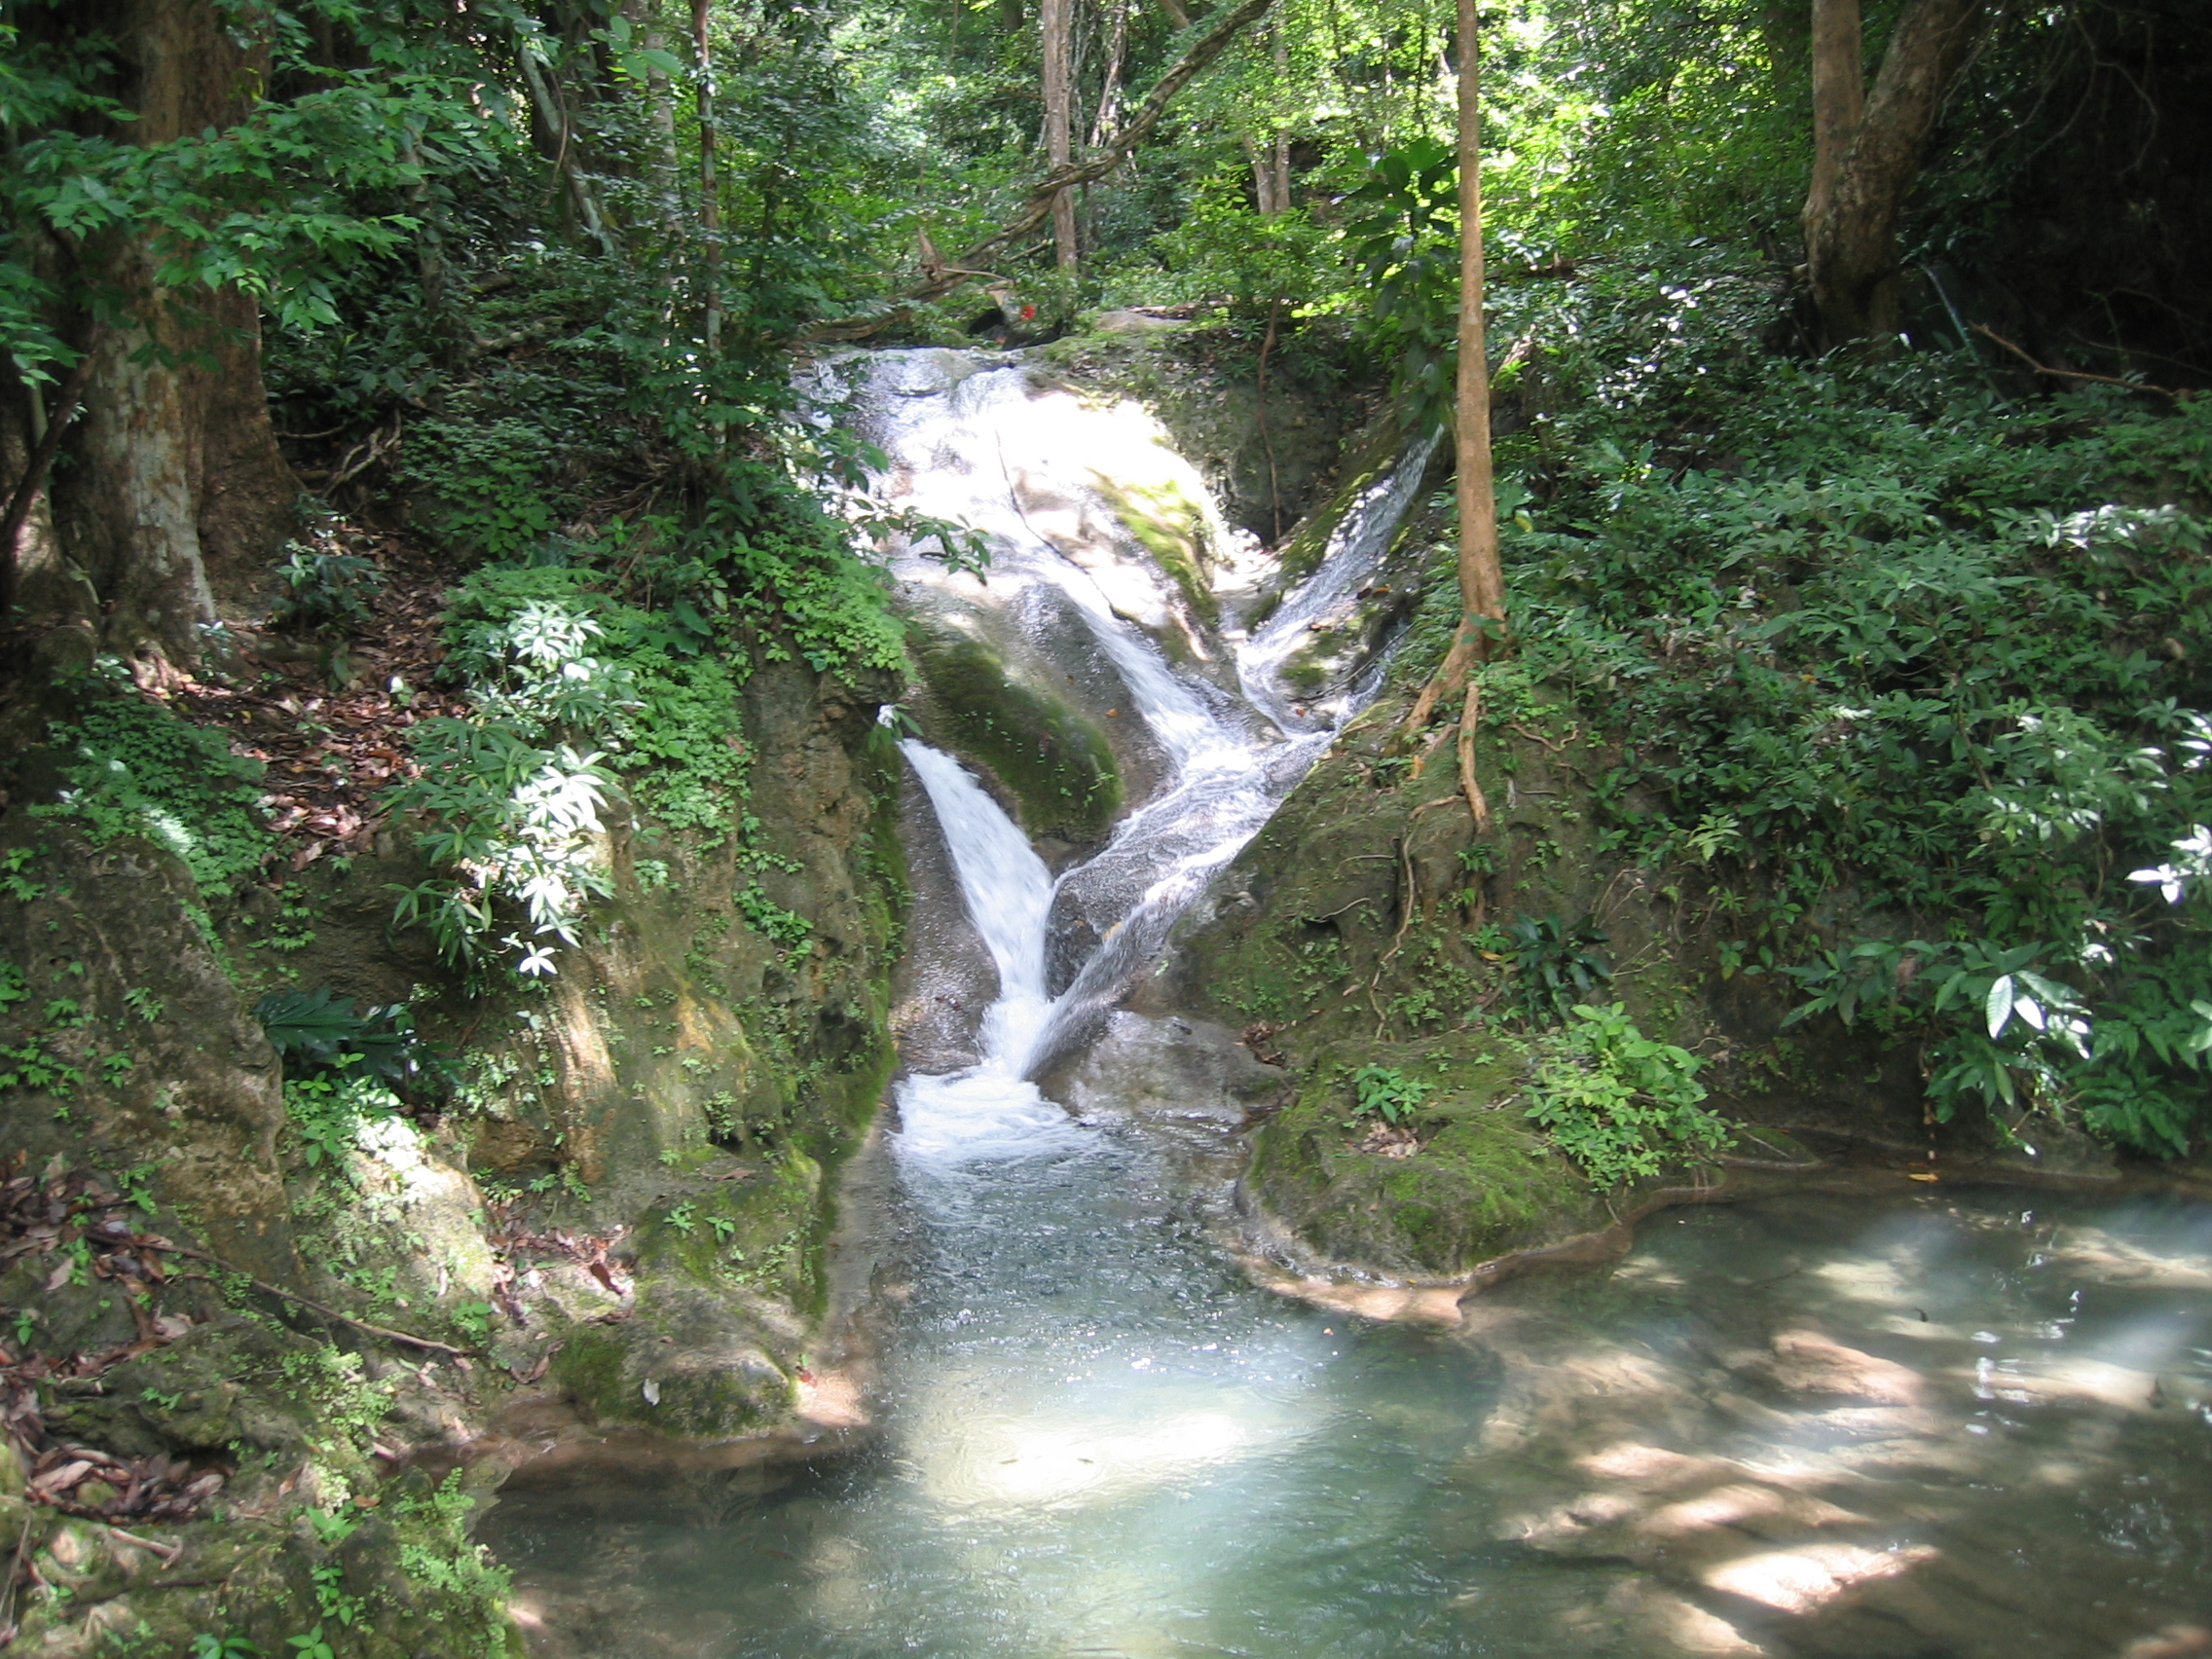
\includegraphics[width=9.7cm]{articles/Kanchanaburi/1437.jpg}
Un p'tit tobogan.

\hspace*{-0.45cm}
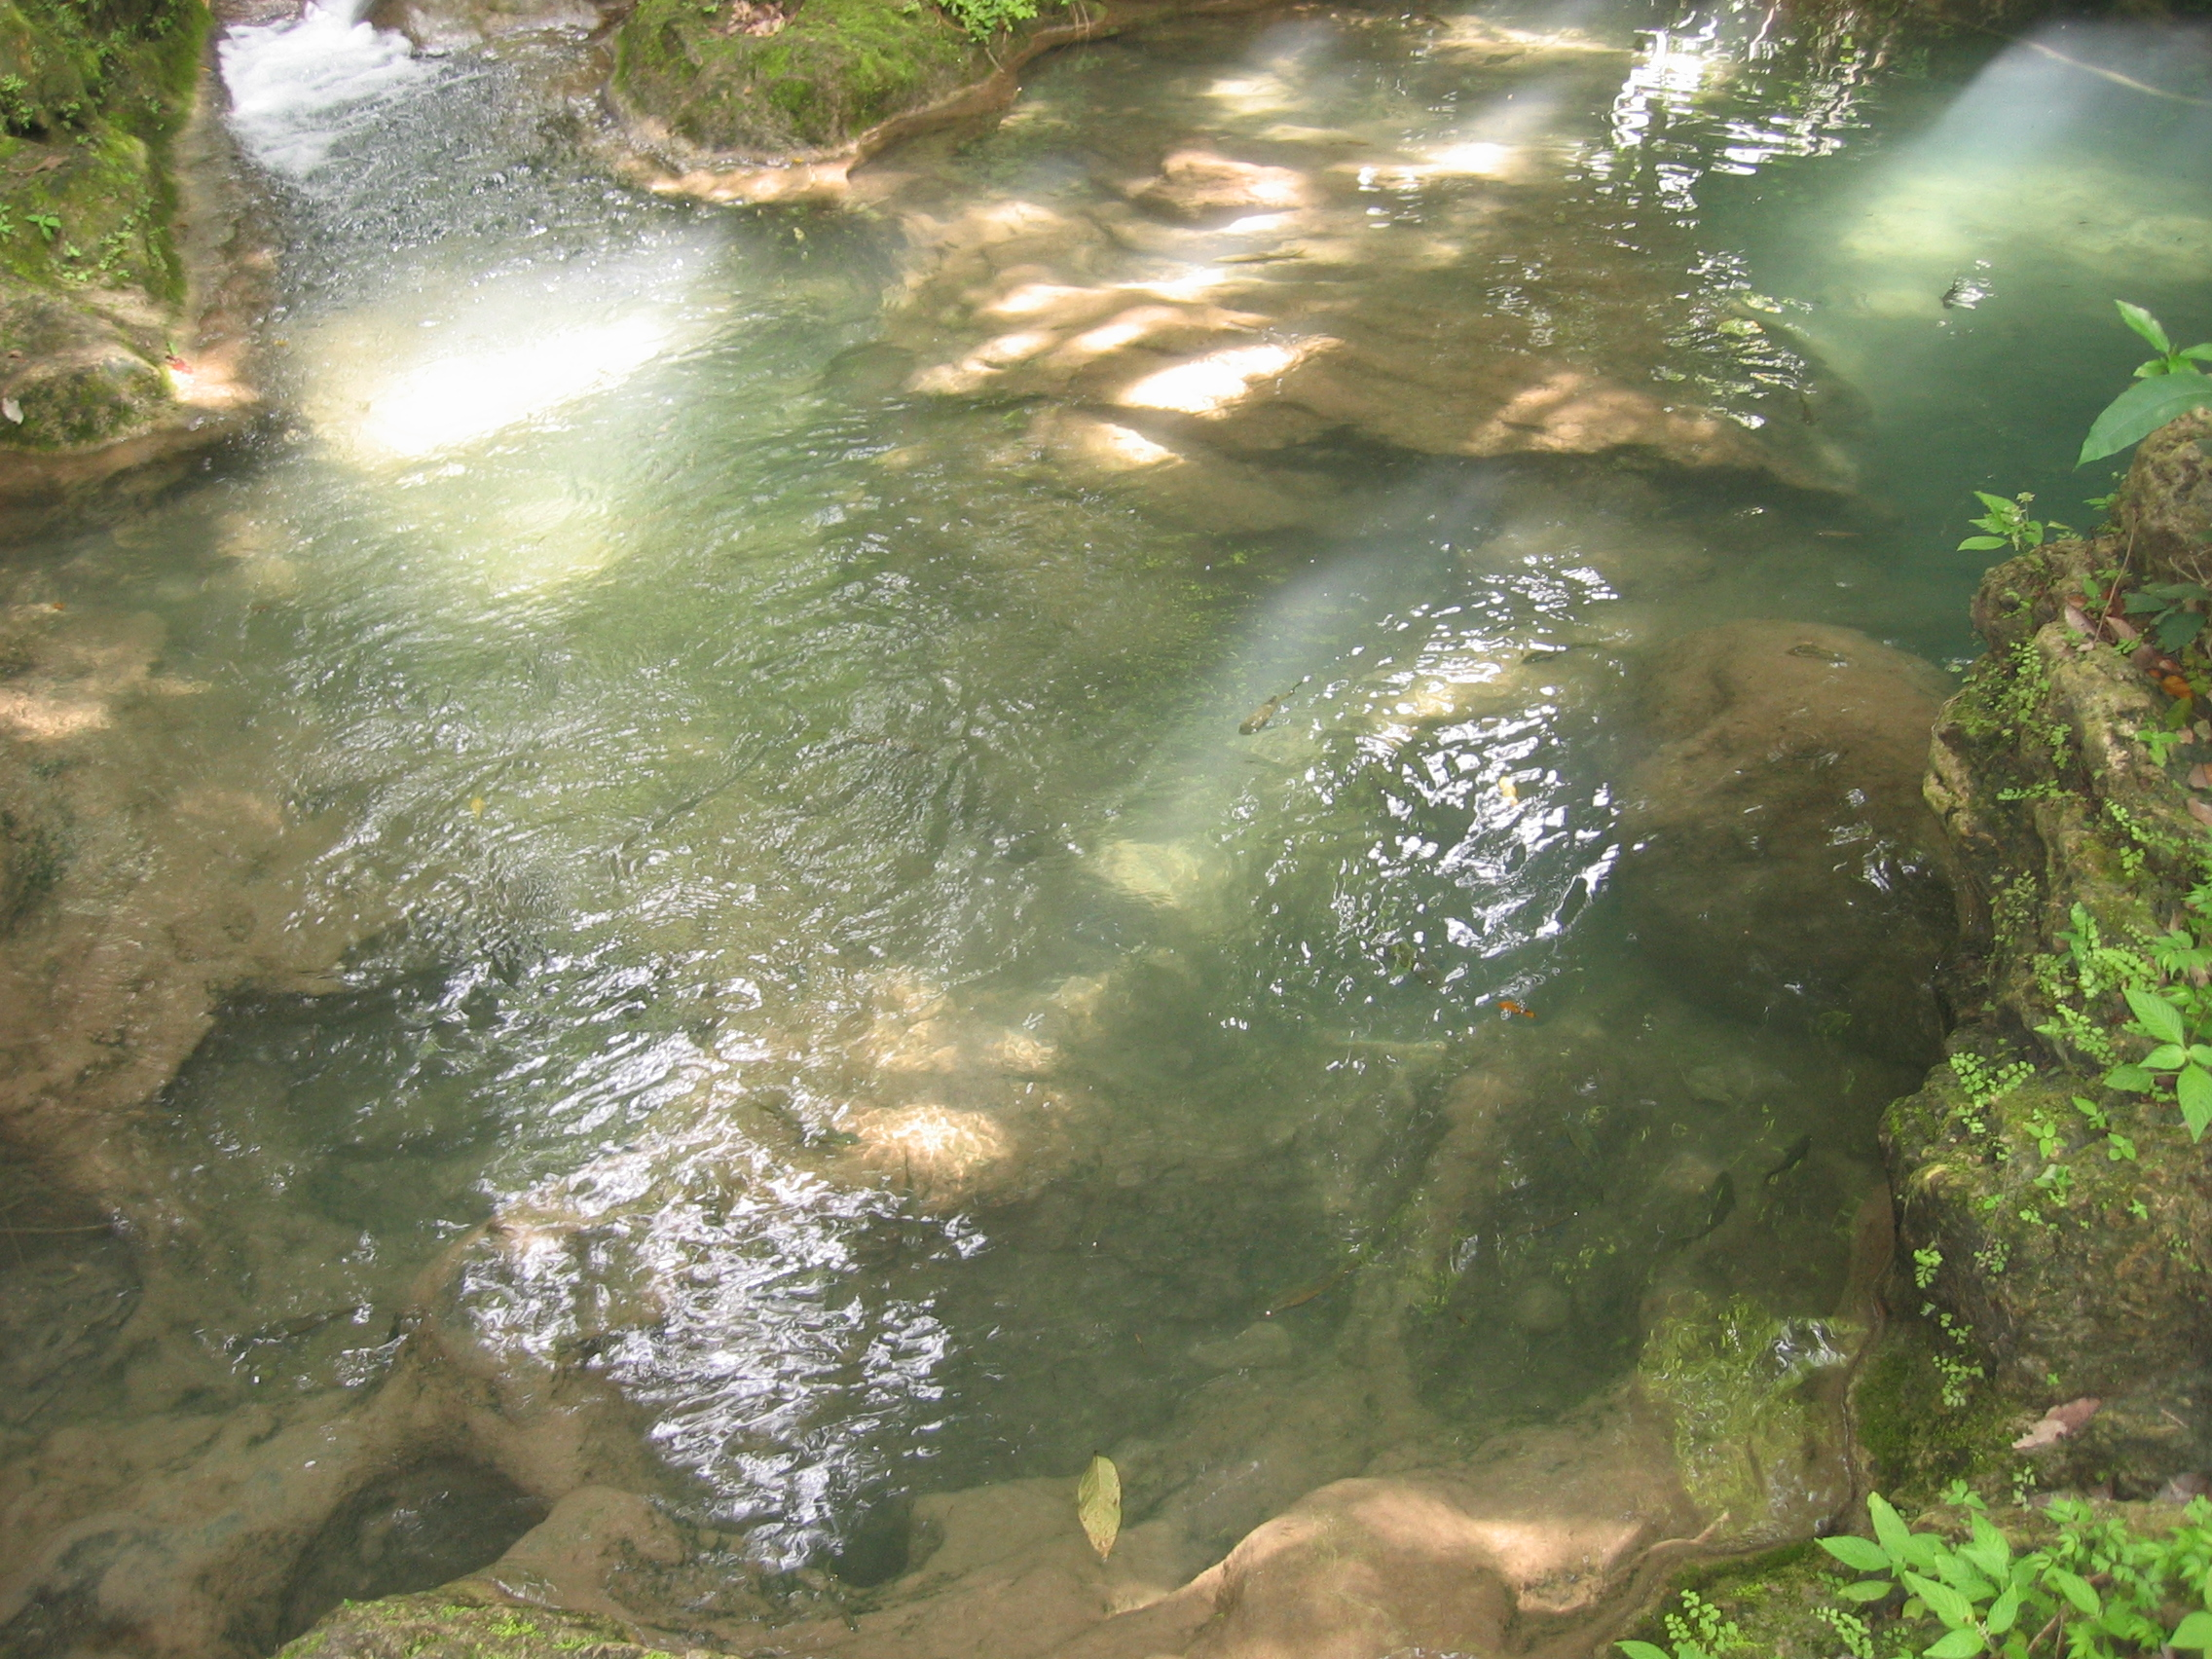
\includegraphics[width=9.7cm]{articles/Kanchanaburi/1438.jpg}
Et un bassin.

Bon, y a quand meme un truc qu'il faut vous dire. Dans tous les bassins, il y a des poissons. Et alors? me direz vous. Un poisson, c'est sympa, mais quand ça a faim, ça l'est moins. Ajoutez à cela un appetit particulier pour les talons d'européens et vous en tirez une sensation assez spéciale qui a un arrière goût de n'y reviens pas. La seule solution était donc de bouger sans arrêt dans l'eau, et on a finit par trouver un petit bassin/jacousie ou y en avait pas.

\begin{dialogue}
  \speak{Moi} Bon c'est bien beau tout ca, mais le dernier bus est à quelle heure?
  \speak{Anna} A 16h
  \speak{Moi} Et il est ?
  \speak{Anna} 16h05...
\end{dialogue}

On essaie de voir avec un groupe de 4 personnes qui avaient loué un tuk tuk collectif (ca passe à 7 largement dedans). Pas moyens. Et là notre négociatrice en chef (Anna) demande a un Thaï qui a un pick-up si il va a Kanchanaburi, il y va, il peut nous emmener. Et c'est parti pour faire le retour dans son coffre, les cheveux au vent (et un peu à la pluie), sympa l'expérience.

Et apres Kanchanaburi me direz vous, c'est vrai que ca fait un bout de temps que vous n'aviez pas nouvelles. J'ai pris le bus pour Ayutaya, au nord de Bangkok, mon but était d'aller à Chiang Mai sans repasser par Bangkok. Je me suis donc arrêté une journée dans la petite ville d'Ayutaya, et y ai loué un velo pour me ballader. J'ai ensuite pris un bus pour Chiang Mai de nuit (10h de route, on s'est fait offrir le cafe à 6h du mat' en arrivant). Et me voici donc a Chiang Mai pour une semaine environs, avant d'aller au Laos. Ma première expérience de la journée à Chiang Mai est une amande mise par un flic hilard alors que je voulais tourner à droite en motor bike là où c'était interdit. J'ai du le suivre au commissariat pour récupérer mon permis, et là, comme par hasard, l'interdiction de tourner à droite ne s'applique plus... Ca me rappelle Bali tout ça.

Voila, l'article est finit, vous pouvez éteindre votre ordinateur et reprendre une activité normale.

%\end{multicols}

\bigskip
\textbf{\textsc{Commentaires}}

 \medskip
Peggy a écrit le 12 juin 2008 :
\begin{displayquote}
ah! de la lecture, des images, des vidéos!! tout ce que l'on aime...
quel grand périple, mais, tu rentres qd (si tu rentres un jour!!) :p
Bisous
Take care!
2+9=11
\end{displayquote}

 \medskip
Etienne a écrit le 13 juin 2008 :
\begin{displayquote}
Je rentre vers mi juillet, je ne sais pas encore precisement car je n'ai pas encore pris mon billet, le tout est que je trouve un appart a Paris avant le debut de mon stage, le 11 aout.
D'ici la, Laos... et retour a Bali.
\end{displayquote}

 \medskip
Jaco a écrit le 14 juin 2008 :
\begin{displayquote}
Eh ben mon ptit Dud, on se la coule douce pendant que d'autres travaillent !
En tout cas profite bien des merveilles de l'exostisme...
Jaco ;)
\end{displayquote}

 \medskip
Titou a écrit le 15 juin 2008 :
\begin{displayquote}
Bali quand tu nous tiens .... :p
Ralala tu n'es vraiment qu'un petit salopiaud ! Dire que y en a qui sont a l'agonie et sous des tonnes de taff.... pff t'es cruel !
Profites mon pti profites !
Merci encore pour ces images et commentaires et fais toi bien plaiz !
A plus ti dud et take care !
ps : Bali ... pourquoi bali ?? ... :p
\end{displayquote}

 \medskip
Nicoz a écrit le 19 juin 2008 :
\begin{displayquote}
Salut ptit Dud,
Alors tu vois que je te met des com aussi en plus de te parler sur MSN :p
Bon d'accord j'avoue jle fais pas à chaque fois mais bon.
Sinon bah profite bien du Laos j'attend les photos et profite bien de Bali et de l'exotisme local ;)
Bonne continuation de ton périple.
Moi jserais toi jsais pas si je reviendrai pour retourver la grisaille parisienne :p
\end{displayquote}

 \medskip
Organisatrice de stages a écrit le 20 juin 2008 :
\begin{displayquote}
bonjour,
chose promise, chose due... même si cela a tardé un peu, je viens de jeter un oeil à votre blog. (en rappel d'un précédent mail : je ne sais pas si cela fera causer vos copains ? vous me direz).
La lecture de votre texte sur Kanchanaburi me donne bien envie de lire plus. Dès que je me serai débarrassée de tous les étudiants récalcitrants (je maintiens ;-)), je ferai une petite pause lecture...
j'en profite aussi pour autre chose : j'ai reçu de Thailande une carte ANONYME ce matin. Comme, contrairement à la plupart des courriers anonymes, elle était plutôt sympa :) Alors merci beaucoup pour le geste.
Bonne continuation dans vos tribulations,
\end{displayquote}

 \medskip
Etienne a écrit le 22 juin 2008 :
\begin{displayquote}
Oups... j'ai pas signe
\end{displayquote}


